\newcommand{\timestack}[0]{\textit{timestack} }

\paragraph{}Os métodos apresentados no Capítulo 2 agora serão utilizadas em conjunto para estimar a altura de ondas do mar. Este algoritmo é composto de três etapas: o pré-processamento, o processamento principal, e a análise da imagem resultante. Estas etapas serão detalhadas nas seções a seguir.
\section{Aparato Instrumental}
Está esquecendo do seu trabalho de projeto integrado. Trazer ele para cá fazendo referência ao seus colegas co-autores.
\section{Pré-Processamento}

\paragraph{}A etapa de pré-processamento tem como objetivo transformar os dados de entrada (o vídeo capturado de uma praia) em uma imagem \timestack tal como ilustrado na Figura \ref{FigDiagramaPreProc}. Acho que o resultado final precisa ser renomeado,pois esse timstack foi gerado no segundo passo do pipeline. Sugiro repensar o nome e corrigir as figuras. Para este fim, são realizados cinco passos: estabilização do vídeo, geração do timestack, conversão para nível de cinza, detecção e remoção do céu. O passo mais importante nessa etapa é a criação do \timestack, que é uma representação espaço-temporal de um vídeo. Os demais passos servirão para garantir a confiabilidade do \timestack e o prepararão para a etapa de processamento principal.  Estas etapas são explicadas nas seções a seguir.
\begin{figure}[h]
\begin{center}
  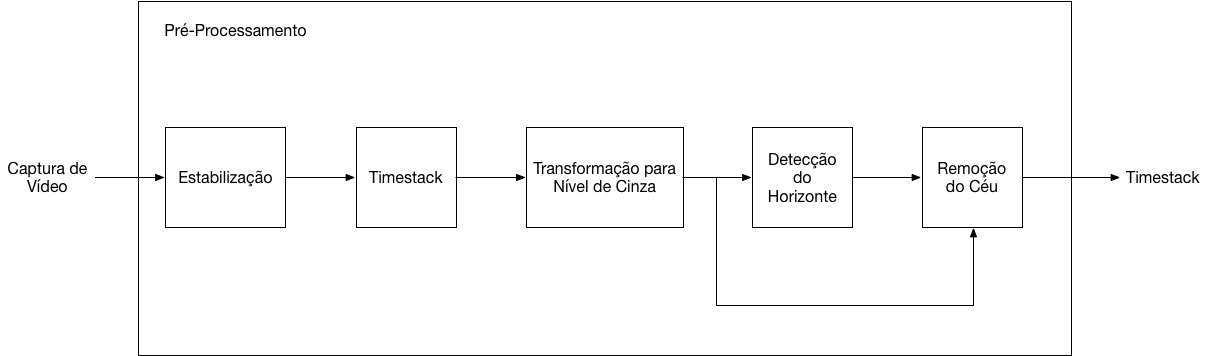
\includegraphics[width=\textwidth,height=\textheight,keepaspectratio]{diagrama_preprocessamento.png}
  \caption[\small{Diagrama de Bloco da etapa de pré-processamento.}]{\label{FigDiagramaPreProc} \small{Diagrama de Bloco da etapa de pré-processamento.}}
\end{center}
\end{figure}
Fazer um parágrafo que descreva de forma geral todo o pré-processoamento. Nas seções em seguida, você fará o aprofundamento.
\section{\textit{Timestack}}
\paragraph{}Um \timestack é uma representação bidimensional de um vídeo, isto é, trata-se de uma forma de transformar tal vídeo em uma só imagem. O \timestack é útil para analisar tais vídeos pois é possível olhar para uma sequencia completa de quadros observando uma única imagem. Dessa forma, pode-se aplicar métodos de processamento de uma única imagem  \timestack, em vez de todo o vídeo.
\paragraph{}Para construir um \timestack, é necessário fixar uma das dimensões espaciais de cada imagem do vídeo, obtendo assim um conjunto de funções unidimensionais. O \timestack deste vídeo é definido então como uma função bidimensional \(s_{Y}(x,t)\) ou \(s_{X}(t,y)\), onde \(x\) e \(y\) são coordenadas espaciais; \(t\) é uma coordenada temporal; as amplitudes \(s_{X}\) e \(s_{Y}\) são a intensidade ou nível de cinza do vídeo \(g(x,y,t)\) quando são fixados os valores \(x = X\) e \(y = Y\), respectivamente. Dessa forma, a relação entre um \timestack e um vídeo é dada por: \(s_{Y}(x,t)=g(x,Y,t)\) e \(s_{X}(t,y) = g(X,y,t)\).
\paragraph{}Note que, na prática, a coordenada temporal \(t\) cumpre o papel de uma coordenada espacial quando o \timestack é exibido como uma imagem, mas sua interpretação continua sendo temporal. É claro que a perda de uma dimensão resulta em perda de informação no vídeo, entretanto, nos casos em que o vídeo é constante na dimensão espacial fixada não a perda de informação. Expandindo esse conceito, nos casos em que o vídeo varie muito pouco em uma de suas dimensões espaciais, não há necessariamente uma perda de conteúdo significativa.
\paragraph{}A análise de ondas marítimas apresenta condição similar a descrita anteriormente. Com a posição da câmera escolhida com cuidado, isto é, xxxxxxxDescrever Tecnicamentexxxxxxxx. Assim, uma onda quebrando ocupará maior parte horizontal da imagem. Além disso, não é importante para a análise desejada entender o tamanho horizontal da onda, apenas o seu tamanho vertical. Precisa-se apenas determinar o seu ponto mais baixo e seu ponto mais alto. Sendo assim, o \timestack mostra-se um método adequado de análise de vídeos para esse projeto.
\begin{figure}[h]
\begin{center}
  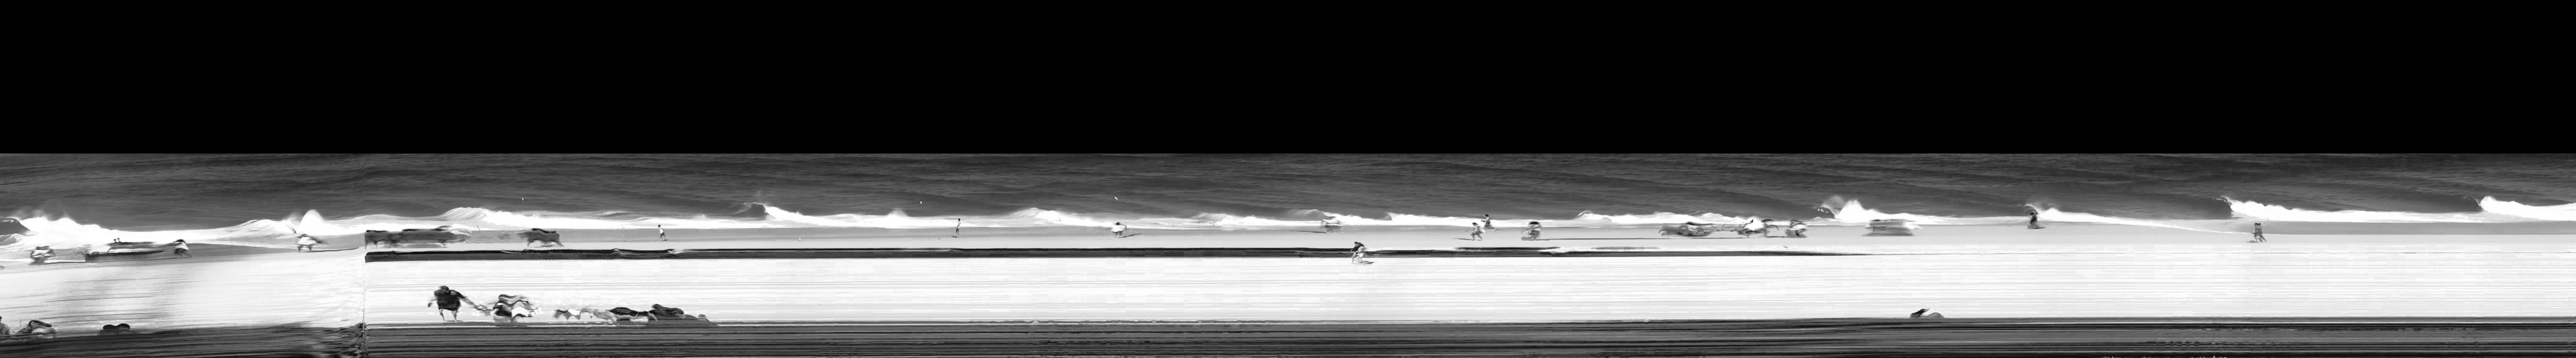
\includegraphics[width=\textwidth,height=\textheight,keepaspectratio]{timestack.jpg}
  \caption[\small{Timestack em nível de cinza gerado a partir de um vídeo estabilizado de uma praia.}]{\label{FigTimestack} \small{Timestack de uma praia.}}
\end{center}
\end{figure}
Explicar a figura chamando a atenção para os detalhes descritos nesta seção.
\section{Estabilização de Vídeo}
\paragraph{}A estabilização de vídeo é fundamental para a criação de um \timestack fiel ao cenário real. Como o \timestack é criado selecionando a coluna central de cada frame do vídeo, é importante que esta coluna corresponda ao mesmo conjunto de pixels de quadro a quadro. Caso a câmera se desloque horizontalmente no decorrer do vídeo, o conjunto de pixels não será o mesmo, e com isso o \timestack formado não será uma representação fiel em duas dimensões do vídeo capturado. A estabilidade na direção vertical é importante para que a estimativa de altura das ondas seja fiel a altura real. Um deslocamento vertical da câmera resulta em um deslocamento das colunas do \timestack, que por sua vez podem imbutir erros na identificação dos pontos de máximo e mínimo de cada onda.
%TODO: Explicar como é feito a estabiliação de vídeo, Colocar exemplo de timestack corrigido e não corrigido para facilitar o entendimento.
\paragraph{}
\section{Conversão para Nível de Cinza}
\paragraph{}Após gerar o \timestack, o mesmo é convertido para nível de cinza. Os passos e etapas subsequentes do algoritmo ora proposto não necessitam trabalhar com cores, apenas a intensidade de cada \textit{pixel} é necessária para estimar a altura das ondas. Com isso, o algoritmo usa mesmo memória e é capaz de ser executado mais rapidamente. Faltou algo nesta última frase.
\paragraph{}A conversão para nível de cinza é realizada de acordo com a seguinte fórmula \cite{Griffith14}:
\[
        I(t, v) = 0.35R(t, v) + 0.5G(t, v) + 0.15B(t, v)
\]
\noindent{}onde \(I(t,v)\) é a intensidade do pixel na posição \((t,v)\) na imagem convertida, e \(R(t,v)\), \(G(t,v)\) e \(B(t,v)\) são, respectivamente, os valores das componentes vermelhas, verdes e azuis do pixel \((t,v)\) da imagem original.
\section{Detecção da Linha de Horizonte}
\paragraph{}Uma etapa importante é a detecção da linha de horizonte a fim de viabilizar a detecção e remoção do céu na imagem. Esta operação é utilizada para facilitar o passo de \textit{thresholding} na etapa de processamento de imagem. Forneça mais detalhes sobre porque isso é importante, possivelmente trazendo inclusive imagens de threshold ruins por conta do fundo de imagem menos intenso.
\paragraph{}A detecção do céu é realizada utilizando um detector de bordas de Canny para identificar a linha do horizonte (Figuras \ref{FigTimestackSkyCanny}). Então, procura-se a primeira borda detectada pelo método de Canny, e todos os pixels acima dessa borda são considerados como pixels do céu.
\begin{figure}[h]
\begin{center}
  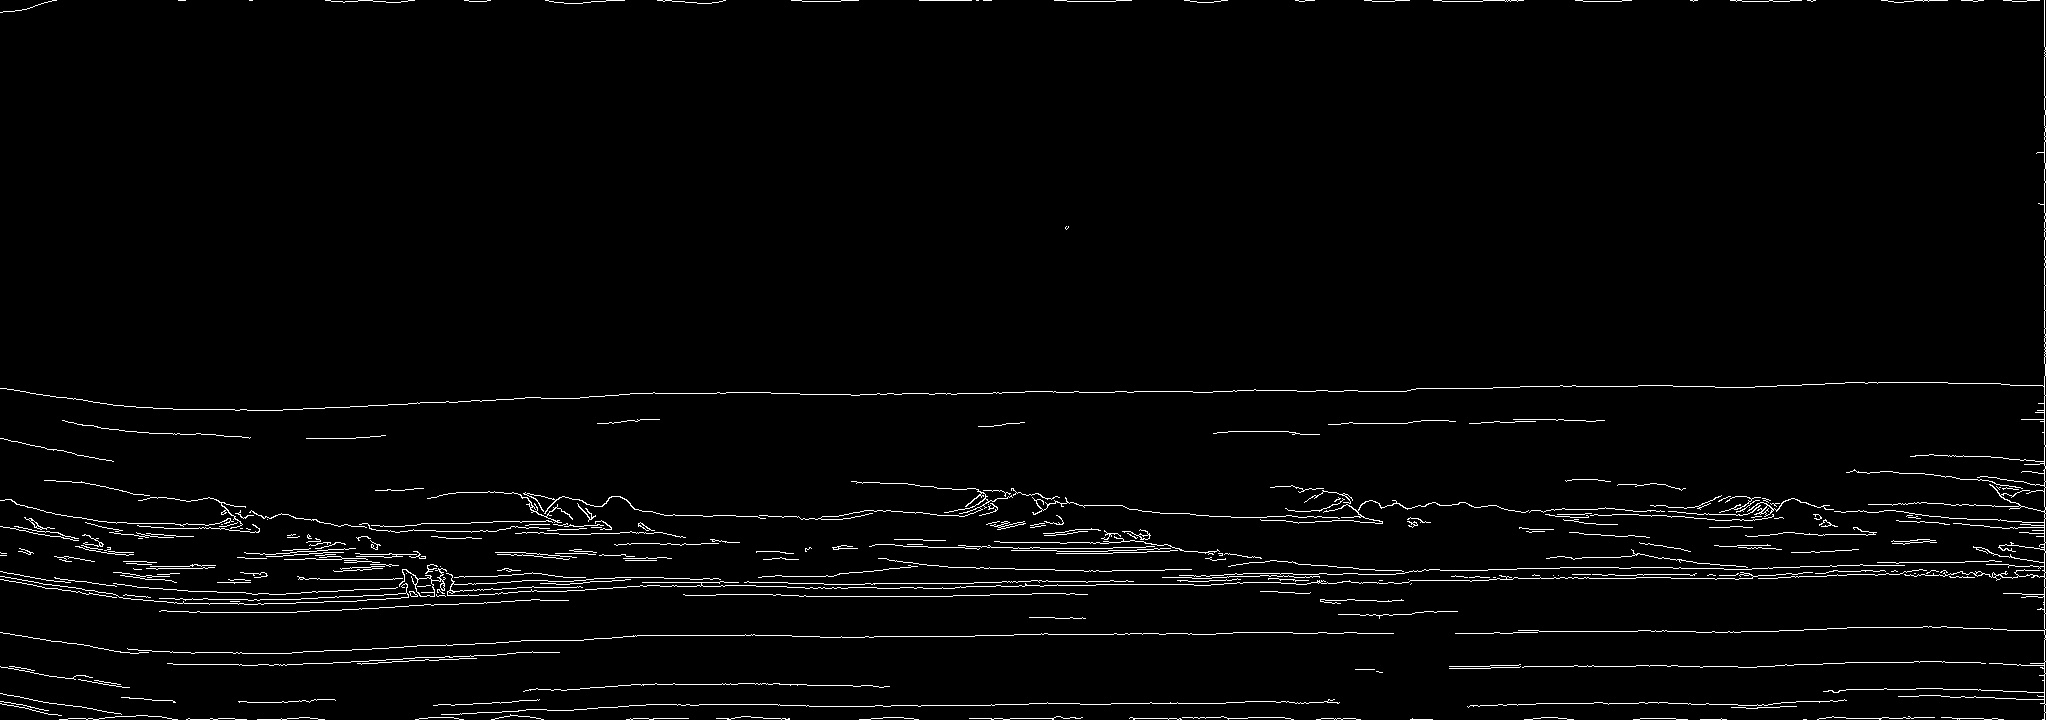
\includegraphics[width=\textwidth,height=\textheight,keepaspectratio]{skydetector_after_canny.jpg}
  \caption[\small{Timestack com bordas detectadas pelo método de Canny. A primeira borda identificada é a linha do horizonte.}]{\label{FigTimestackSkyCanny} \small{\textit{Timestack} com bordas detectadas.}}
\end{center}
\end{figure}
\section{Remoção do Céu}
\paragraph{}O último passo da etapa de pré-processamento é a remoção do céu. Este passo utiliza duas entradas, a linha do horizonte detectada pelo passo anterior, e o \timestack em nível de cinza. A partir da linha do horizonte, considera-se todos os pixels do \timestack em nível de cinza acima dessa linha como preto. Este passo é importante pois o nível médio de intensidade do céu pode variar muito dependendo do nível de iluminação no momento que o vídeo foi capturado. Os dois principais fatores que impactam o nível de iluminação são as condições climáticas (dias mais nublados ou mais claros alteram o nível de intensidade médio do céu) e o horário do dia (o nível de iluminação será diferente no começo da manhã quando comparado com o meio do dia).
\paragraph{}Sem a remoção do céu, é difícil definir um valor automático de \textit{threshold} que será utilizado na etapa de processamento principal. Uma tarefa essencial é ser capaz de separar o céu, o mar e a faixa de espuma da arrebentação. Com o céu removido, ao operação de  \textit{threshold} produzirá resultados mais adequados para dar suporte às etapas de medição.
\section{Processamento Principal}
\begin{figure}[h]
\begin{center}
  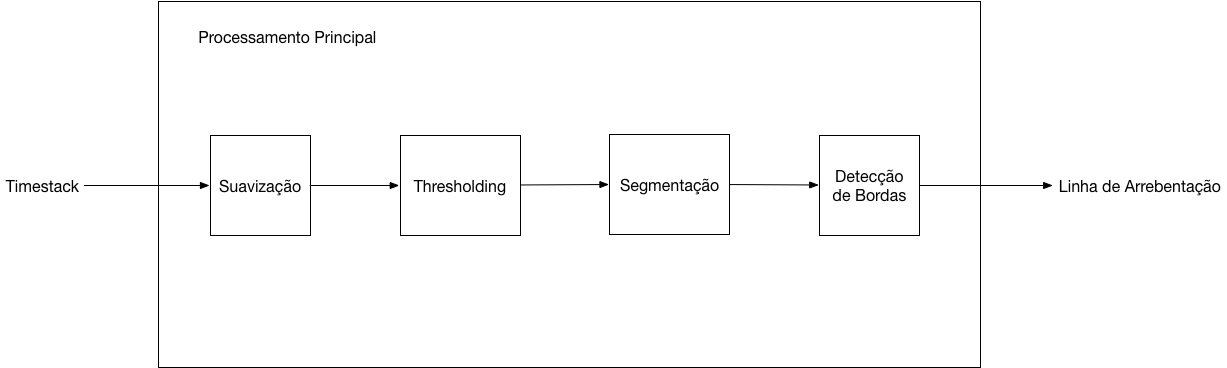
\includegraphics[width=\textwidth,height=\textheight,keepaspectratio]{diagrama_processamento.png}
  \caption[\small{Diagrama de Bloco da etapa de processamento principal.}]{\label{FigDiagramaProc} \small{Diagrama de Bloco da etapa de processamento principal.}}
\end{center}
\end{figure}
\paragraph{}A etapa de processamento principal tem como objetivo extrair a linha de arrebentação (figura \ref{FigLinhaArrebentacao}) de um \timestack gerado pelo pré-processamento. A linha de arrebentação é definida como a linha que delimita a região de espuma, formada depois das ondas quebrarem, do restante do mar atrás das ondas. A forma que essa linha evolui, ou seja, o seu formato, como e quanto a linha sobe ou desce indica tanto a localização das ondas como a sua altura. Esta frase está confusa, reescrever. Além disso, como foi mostrado anteriormente, a localização das ondas no \timestack representa a sua localização temporal no vídeo capturado, e desta forma é possível calcular a periodicidade das ondas.
\begin{figure}[h]
\begin{center}
  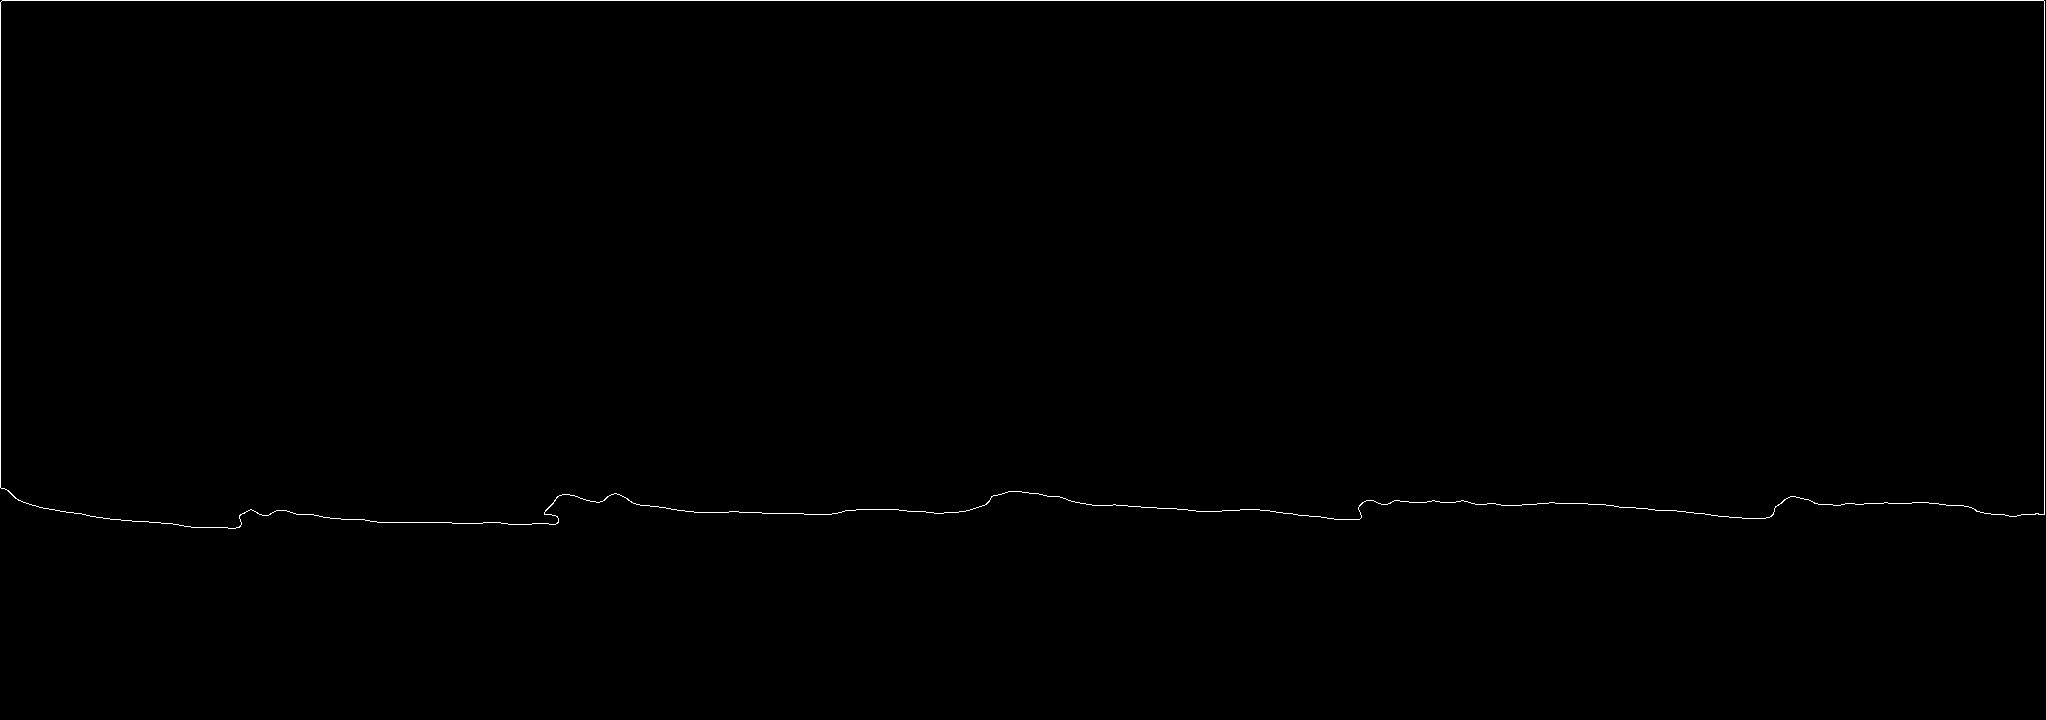
\includegraphics[width=\textwidth,height=\textheight,keepaspectratio]{mainprocessing_breakzone_line.jpg}
  \caption[\small{Linha de arrebentação detectada pelo processamento principal.}]{\label{FigLinhaArrebentacao} \small{Linha de arrebentação detectada pelo processamento principal.}}
\end{center}
\end{figure}
\section{Suavização}
\paragraph{}A primeira etapa de suavização é realizada utilizando um filtro passa-baixas gaussiano, implementado no domínio do espaço com máscara de tamanho 15. Porque este valor? Este efeito de suavização é importante para reduzir o nível de ruído na imagem, facilitando a identificação das bordas relevantes nos passos subsequentes. 
Outro efeito desejado é homogeneizar o nível de intensidade das regiões da imagem, de forma que o passo de \textit{thresholding} consiga segmentar a região de espuma do \timestack de forma mais consistente.
%TODO: Adicionar imagem da primeira suavização
\section{\textit{Thresholding}}
\paragraph{}\textit{Thresholding} é o primeiro passo para realizar a segmentação. Neste passo separa-se a região de espuma do restante do mar, alterando todos os pixels com intensidade acima de 150 para 0 O valor não é dinâmico por conta daquela história de remoção do céu (figura \ref{FigThreshold}). 
\begin{figure}[h]
\begin{center}
  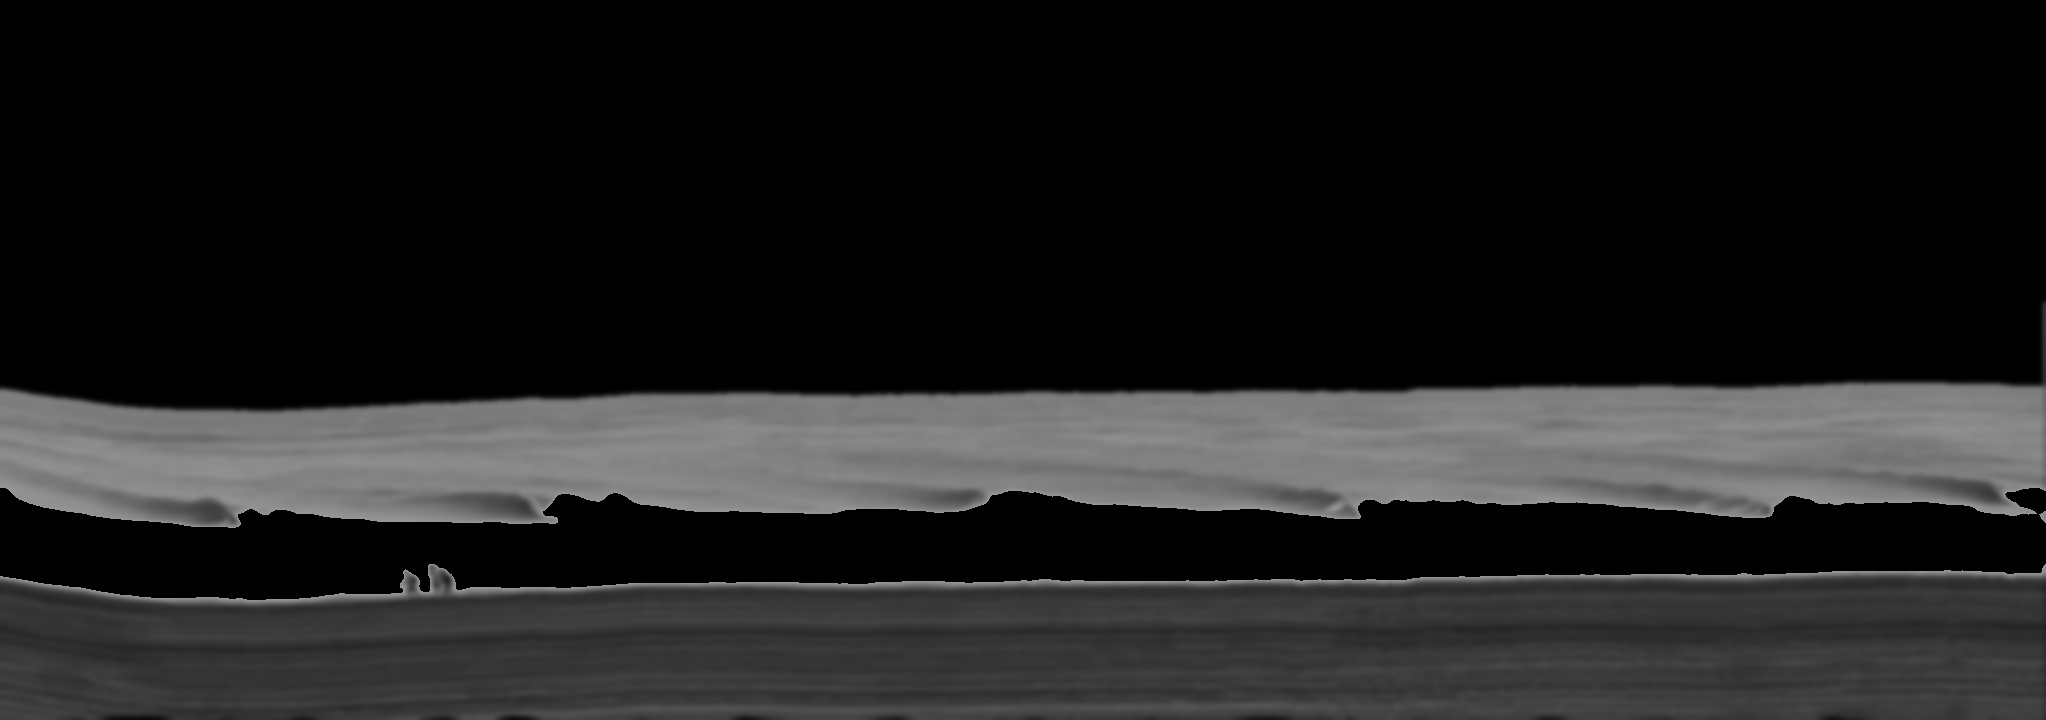
\includegraphics[width=\textwidth,height=\textheight,keepaspectratio]{mainprocessing_threshold.jpg}
  \caption[\small{\textit{Timestack} após aplicação de um \textit{threshold}.}]{\label{FigThreshold} \small{\textit{Timestack} após aplicação de um \textit{threshold}.}}
\end{center}
\end{figure}
\section{Aumento de Nitidez e Suavização}
\section{Detecção de Bordas}
\section{Segmentação}
\section{Detecção de Bordas}
\section{Análise e Indentificação das Ondas Marítimas}
\paragraph{}A última etapa do algoritmo de estimação da altura de ondas do mar é analisar a linha de arrebentação extraída do \timestack e identificar as ondas do mar presentes nesta imagem. Feito isso, é possível encontrar o ponto mínimo e máximo locais da linha de arrebentação, que correspondem ao ponto mínimo e máximo da onda em questão.
\begin{figure}[h]
\begin{center}
  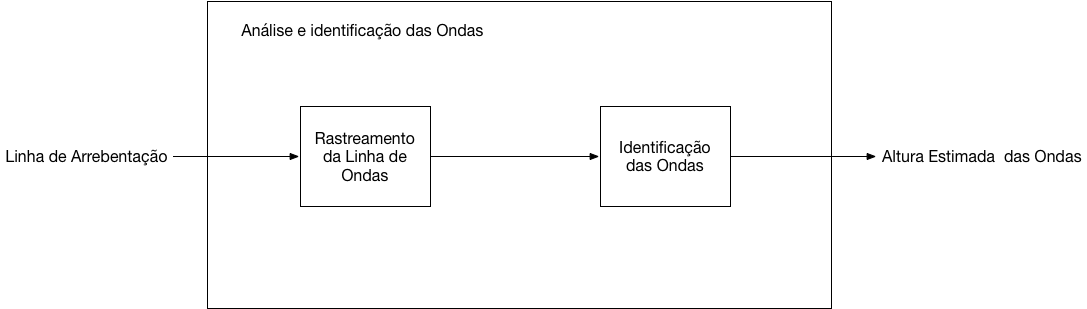
\includegraphics[width=\textwidth,height=\textheight,keepaspectratio]{diagrama_analise.png}
  \caption[\small{Diagrama de Bloco da etapa de análise. Fonte: Autor}]{\label{FigDiagramaAnalise} \small{Diagrama de Bloco da etapa de análise.}}
\end{center}
\end{figure}
\section{Rastreamento da Linha de Ondas}
\paragraph{}O primeiro passo desta etapa consiste em rastrear a linha de arrebentação encontrada, isto é, construir uma sequência \(s[n]\) que indica a sequência ordenada dos pontos \((x,y)\) que compõe a linha de arrebentação. Esta sequência ordenada permite caminhar por cima da linha de arrebentação e assim determinar os pontos de máximo e mínimo locais da linha.
\paragraph{}Para rastrear a linha de arrebentação foi utilizado um algoritmo que, dado um ponto de origem \(s[0] = (x_{i},y_{i})\), encontra o próximo ponto da linha, o adiciona a sequência e busca o próximo ponto, até que não encontre mais nenhum ponto disponível para adicionar na sequência \(s[n]\). o pseudo-código \ref{AlgLineTracking} ilustra o algoritmo de rastreamento, e o pseudo-código \ref{AlgFirstPoint} ilustra o algoritmo que popula o primeiro ponto da sequência $s[n]$. Explicar a idéia que é implementada no algoritmo.
\begin{algorithm}
\caption{Algoritmo de Rastreamento de Linha}
\label{AlgLineTracking}
\begin{algorithmic}
\Procedure{RastreiaLinha}{$raioDeBusca$}
\State $PontoAtual \gets s[N]$ \Comment{último ponto de s[n]}
\For{ pontos p ao redor de $PontoAtual$ em um raio de $raioDeBusca$ } 
        \If { $p \neq 0$ e $p$ não está em $s[n]$ }
                \State $s[N+1] \gets p$
        \EndIf
\EndFor
\If{algum ponto foi adicionado a $s[n]$}
        \State{repetir o procedimento para o último ponto encontrado}
\Else
        \If{$raioDeBusca \leq 3$}
                \State{repetir o procedimento com $raioDeBusca+1$}
        \Else
                \State{fim}
        \EndIf
\EndIf
\EndProcedure
\end{algorithmic}
\end{algorithm}
\begin{algorithm}
\caption{Algoritmo de Identificação do Primeiro Ponto da Linha}
\label{AlgFirstPoint}
\begin{algorithmic}
\Procedure{EncontraPrimeiroPonto}{}
\For{cada coluna $c$ no \timestack}
        \For{cada elemento $e$ na coluna $c$}
                \If{valor do elemento $e > 0$}
                        \State $s[0] = \text{posição do elemento } e$
                        \State{fim}
                \EndIf
        \EndFor
\EndFor
\EndProcedure
\end{algorithmic}
\end{algorithm}
\section{Identificação das Ondas}
\paragraph{}O último passo para estimar a altura das ondas em um \timestack é identificar as ondas na linha rastreada no passo anterior. Para isso, calcula-se a derivada da sequência discreta $s[n]$, da seguinte forma:
\[
        s'[n] = s[n] - s[n-1], \text{para n $>$ 0}
\] 
\noindent{}A sequência $s'[n]$ indica quais trechos da sequência original $s[n]$ são crescentes, decrescentes ou constantes. Então, ao caminhar sobre a sequência derivada $s'[n]$, é trivial determinar quais são as faces crescentes das ondas. Em um cenário ideal, o ponto inicial de uma face crescente corresponde ao ponto mínimo local de uma onda, e o último ponto crescente desta face corresponde ao ponto de máximo local, determinando assim a altura da onda. Entretanto, em uma imagem não ideal podem existir trechos que a derivada é $0$, ou até mesmo negativa, antes da sequência tornar a crescer. A figura \ref{FigAutomato} descreve um autômato que reconhece uma onda considerando as condições descritas anteriormente.
\begin{figure}[h]
\begin{center}
  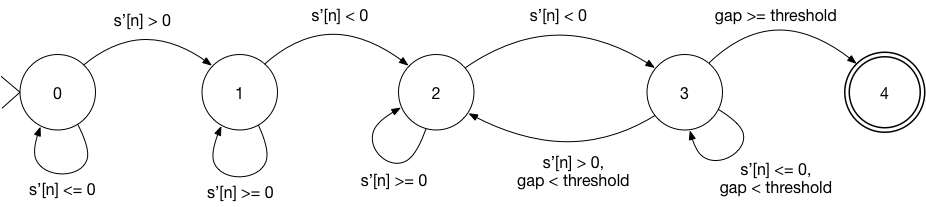
\includegraphics[width=\textwidth,height=\textheight,keepaspectratio]{automato_identificacao_onda.png}
  \caption[\small{Autômato Finito Determinístico que identifica uma onda em uma linha de arrebentação.}]{\label{FigAutomato} \small{Autômato Finito Determinísticoque identifica uma onda em uma linha de arrebentação.}}
\end{center}
\end{figure}
\noindent{}O estado 0 do autômato procura pela primeira derivada $s'[n]$ positiva, marcando o ponto equivalente de $s[n]$ como o mínimo da onda e avançando para o estado 1. O estado 1 procura pela primeira derivada negativa de $s'[n]$, marcando o ponto equivalente de $s[n]$ como candidato ao ponto máximo da onda e andando para o estado 2. Então, os estados 2 e 3 buscam por "buracos" ou \textit{gaps} no trecho de derivada positiva, onde a derivada se torna negativa por um curto período e depois $s[n]$ torna a crescer. O estado 2 procura por novos pontos de máximo, trechos onde a derivada é positiva, e o estado 3 procura por trechos de derivada negativa. Quando o estado 3 encontrar uma derivada positiva, o autômato retorna para o estado 2. Enquanto o estado 3 encontrar derivadas não-positivas um contador de tamanho do \textit{gap} é incrementado. Quando o tamanho do \textit{gap} é superior a um certo limite, o autômato avança para o estado 4, identificando assim que um candidato a uma onda foi encontrado, delimitado pelos pontos de mínimo e máximo encontrados anteriormente. Este candidato apenas será considerado uma onda se sua altura estiver dentro de uma faixa de controle, isto é, são descartadas ondas muito pequenas ou muito grandes.A figura \ref{FigWave} mostra os pares de pontos máximo e mínimo identificados pelo autômato em uma linha de arrebentação aplicados no \timestack original. As linhas vermelhas unem os pares de pontos encontrados. Você vai precisar dar uma ênfase maior na linha vermelha da imagem para ficar nítido.
\begin{figure}[h]
\begin{center}
  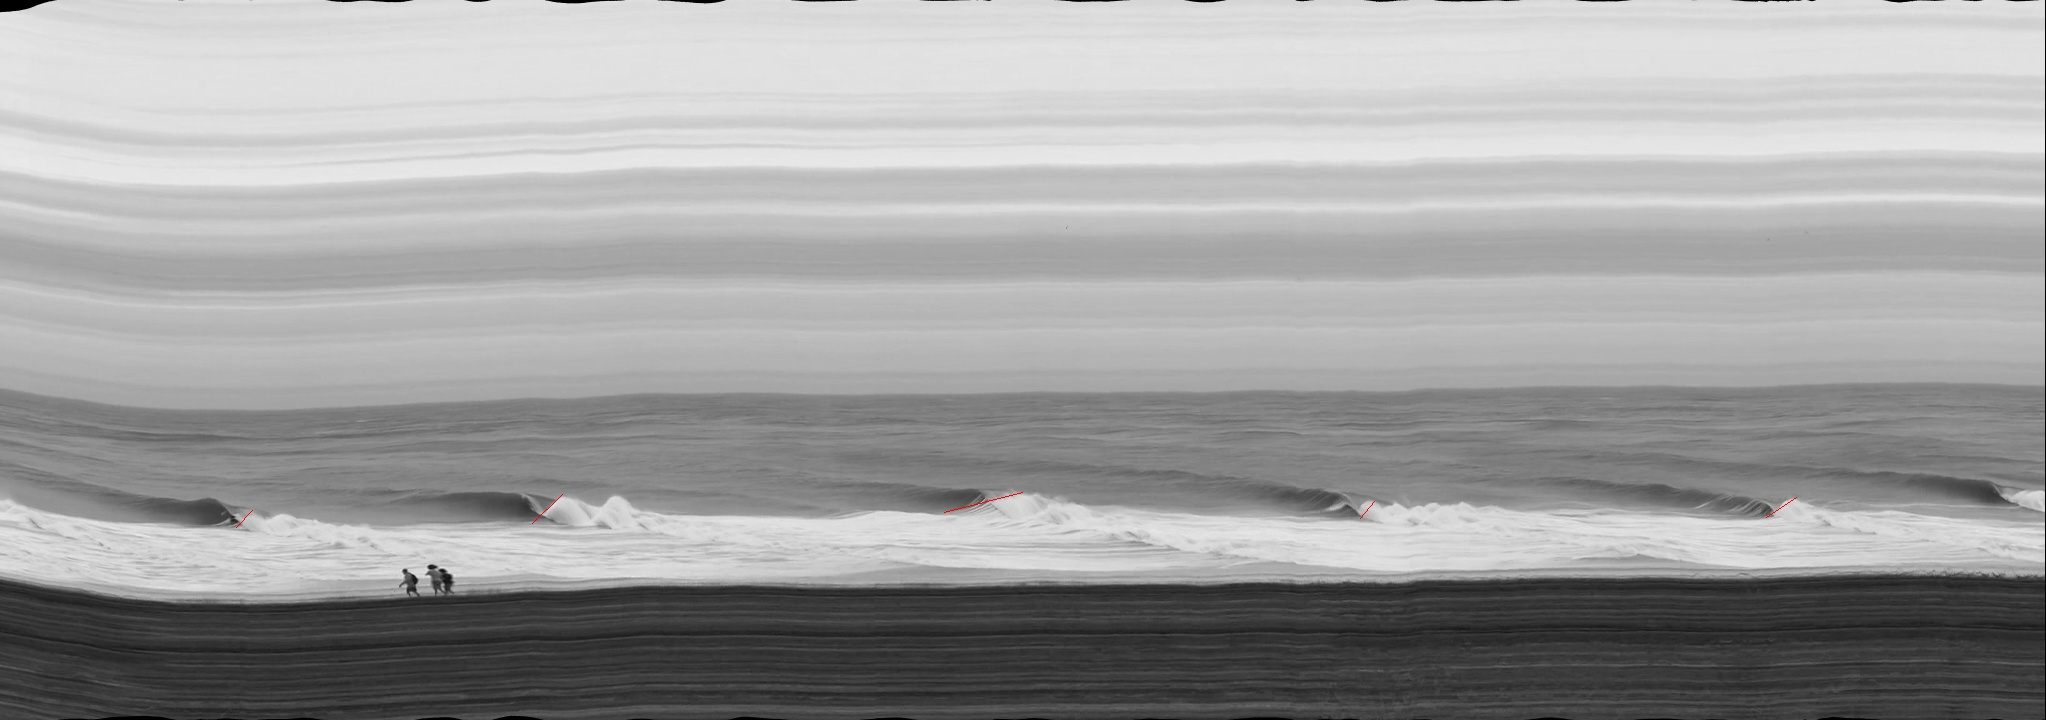
\includegraphics[width=\textwidth,height=\textheight,keepaspectratio]{result_wave.jpg}
  \caption[\small{Ondas identificadas pelo autômato.}]{\label{FigWave} \small{Ondas identificadas pelo autômato.}}
\end{center}
\end{figure}

